% ScholarFlow — Software Engineering Laboratory Project Report
% Main driver file. Compile with: pdflatex main.tex (run twice for TOC)
\documentclass[12pt,a4paper]{article}

% ---------- Encoding & fonts ----------
\usepackage[utf8]{inputenc}
\usepackage[T1]{fontenc}
\usepackage{lmodern}

% ---------- Page layout ----------
\usepackage[a4paper,margin=1in]{geometry}
\usepackage{setspace}
\onehalfspacing

% ---------- Graphics & tables ----------
\usepackage{graphicx}
\usepackage{float}
\usepackage{caption}
\usepackage{booktabs}
\usepackage{longtable}
\usepackage{array}

% ---------- Links & lists ----------
\usepackage[hidelinks]{hyperref}
\usepackage{enumitem}

% ---------- Misc ----------
\usepackage{xcolor}

% ---------- UI screenshot helper ----------
% \uiscreenshot{file}{caption}{label}: includes figures/<file> when present,
% otherwise renders a labeled placeholder box. Drop the PNG in later and it
% picks it up automatically — no .tex change needed.
\newcommand{\uiscreenshot}[3]{%
  \begin{figure}[H]
  \centering
  \IfFileExists{figures/#1}{%
    \includegraphics[width=0.95\textwidth]{figures/#1}%
  }{%
    \fbox{\parbox[c][5cm]{0.93\textwidth}{\centering
      \textbf{[TODO screenshot:] \url{figures/#1}}\\[0.3cm]
      Capture at 280--320\,dpi PNG before submission.}}%
  }%
  \caption{#2}\label{#3}
  \end{figure}
}

\graphicspath{{./}{./figures/}}

\begin{document}

% Title page (edit course/teacher/section placeholders in title.tex)
% Title page — edit the TODO placeholders (course code, section, teacher, group)
\begin{titlepage}
\begin{center}


\includegraphics[width=0.22\textwidth]{uiu.png}\\[0.4cm]
{\large United International University}\\
{\large Department of Computer Science and Engineering}\\[0.6cm]

{\LARGE\bfseries ScholarFlow\\[0.2cm]}
{\large An AI-Powered Research Paper Collaboration Hub}\\[0.8cm]

\begin{tabular}{rl}
Course Title: & Software Engineering Laboratory \\
Course Code:  & CSE 3422 \\
Section:      & K \\
Team Name:    & Phantom Devs \\
\end{tabular}\\[0.8cm]

\begin{tabular}{|l|l|}
\hline
\textbf{Student Name} & \textbf{Student ID} \\
\hline
Md.\ Atikur Rahaman        & 0112310298 \\
Md.\ Salman Rohoman Nayeem & 0112310484 \\
Pratay Paul                & 0112310163 \\
Md.\ Sarowar Alam Sourov   & 0112310302 \\
\hline
\end{tabular}\\[0.8cm]

{\bfseries Project Repository}\\
\url{https://github.com/Atik203/Scholar-Flow}\\

\end{center}
\end{titlepage}


% Front matter
\pagenumbering{roman}
\tableofcontents
\newpage
% Mapped Program Outcomes — adapt wording to your department's PO list
\section*{Mapped Program Outcomes}
\addcontentsline{toc}{section}{Mapped Program Outcomes}

\begin{longtable}{|>{\raggedright\arraybackslash}p{3.6cm}|>{\raggedright\arraybackslash}p{11.6cm}|}
\hline
\textbf{Program Outcome (PO)} & \textbf{Project Alignment} \\
\hline
\endfirsthead
\hline
\textbf{Program Outcome (PO)} & \textbf{Project Alignment} \\
\hline
\endhead
PO2: Problem Analysis &
ScholarFlow addresses fragmented academic research workflows in Bangladesh
(survey of 32 respondents: 46.9\% struggle with notes, 40.6\% cannot find papers
later, tool satisfaction only 3.28/5). The problem was analyzed into computable
requirements for a unified AI-native research hub. \\
\hline
PO3: Design and Development of Solutions &
A secure, scalable platform was designed and built: Next.js frontend, Express
REST API, PostgreSQL + pgvector, AWS S3 storage, multi-provider AI
(Gemini/OpenAI), and role-based workspaces for researchers, team leads, and
administrators. \\
\hline
PO5: Modern Tool Usage &
Modern stack throughout: Next.js 16, React 19, TypeScript, Prisma ORM,
TipTap editor, Stripe billing, Git/GitHub + Turborepo monorepo, Vercel/Render
deployment. \\
\hline
PO8: Ethics &
JWT authentication, bcrypt password hashing, role-based access control,
presigned S3 URLs, Stripe webhook signature verification, and access-checked AI
and search endpoints protect sensitive research data. \\
\hline
PO9: Individual and Teamwork &
Built by the four-member team ``Phantom Devs'' with distributed ownership
(full-stack, backend/database, frontend/QA, AI/presentation) and coordinated
delivery across phased milestones. \\
\hline
PO10: Communication &
System architecture, workflows, and implementation are documented in this report,
the SRS, Figma prototypes (102 screens), and presentation slides for technical
and non-technical audiences. \\
\hline
PO12: Lifelong Learning &
The team independently adopted emerging technologies beyond coursework:
pgvector semantic search, RAG pipelines, Y.js real-time collaboration, and
multi-provider LLM fallback strategies. \\
\hline
\end{longtable}

\newpage
% Abstract — two concise paragraphs, standalone page
\section*{Abstract}
\addcontentsline{toc}{section}{Abstract}

Academic research workflows remain heavily fragmented, forcing students and scholars to juggle disconnected tools for paper storage, PDF reading, note-taking, reference management, and manuscript writing. A requirements survey among academic researchers confirmed substantial productivity loss due to context switching, low satisfaction with legacy reference managers, and universal demand for integrated artificial intelligence assistance. This report presents \textbf{ScholarFlow}, a full-stack, AI-powered research paper collaboration hub designed to unify the end-to-end research lifecycle into a single collaborative platform: cloud document management with automated metadata extraction, semantic search powered by vector embeddings, inline PDF annotations, collaborative TipTap academic writing, and multi-tenant research workspaces.

The platform is engineered as a decoupled TypeScript system comprising a Next.js 16 frontend, an Express.js REST and WebSocket backend, a PostgreSQL database enhanced with pgvector, and an AWS S3 storage infrastructure with presigned access. Integrated multi-model AI orchestration powers contextual summarization, structured Q\&A insights, and multi-paper synthesis under strict workspace access controls, while production-grade billing is managed via idempotent Stripe webhooks. ScholarFlow demonstrates the practical application of software engineering principles---modular design, automated testing (21 test suites / 59 tests), strict type safety, and real-time synchronization---to deliver an accessible, scalable, and secure platform for modern academic collaboration.

\newpage
\pagenumbering{arabic}

% Chapters (one file per chapter — fill in content, replace TODO figures)
\section{Introduction}
Effective research requires finding the right papers, understanding them
quickly, organizing them reliably, and collaborating without friction. In
practice, researchers juggle four to five disconnected tools --- reference
managers, cloud drives, PDF readers, note-taking apps, and general chatbots
--- losing context at every switch. Cognitive-load research and the
ScholarFlow survey agree on the cost: the average researcher uses 4.2
disconnected tools daily, context-switching overhead cuts productivity by
30--50\%, and current tool satisfaction sits at only 3.28 out of 5.

ScholarFlow was developed to consolidate this fragmented workflow into one
AI-native hub: upload and organize papers, read and annotate them, write with
integrated citations, and collaborate in shared workspaces with real-time
co-editing. Unlike legacy tools that treat AI as an optional add-on,
ScholarFlow makes AI a first-class capability of every workflow --- semantic
search instead of keyword search, generated summaries and Q\&A instead of
manual skimming, and contextual writing assistance instead of a detached
chatbot window.

This document serves four audiences. The \emph{development team} finds
architectural blueprints and implementation rules for the multi-tier system
(Next.js frontend, Express backend, PostgreSQL with pgvector). \emph{Project
evaluators} find scope boundaries, phased delivery evidence, and measurable
acceptance criteria. The \emph{quality assurance} view is covered by testable
requirements and performance budgets (sub-300\,ms semantic search, $<$50\,ms
per server-side query event, 99.9\% availability target). Finally,
\emph{stakeholders} find market validation --- a 32-respondent survey with
75\% need confirmation and 100\% AI-feature interest --- together with a
freemium revenue model designed for student affordability.

Development followed an Agile-iterative life cycle across phased rollouts:
an MVP slice (authentication $\rightarrow$ upload $\rightarrow$ library
$\rightarrow$ editor $\rightarrow$ sharing) first, then AI capabilities on
top of the library, then collaboration and real-time features, then
monetization and administration, closing with hardening and launch readiness.
Each phase shipped a thin vertical slice rather than broad incomplete
scaffolding, with continuous gates --- build, type-check, lint, and tests ---
required green on every merge. The project applies core software engineering
principles throughout: modularity (decoupled frontend/backend monorepo),
scalability (pooled connections, paginated and access-scoped queries),
maintainability (strict TypeScript, Zod contracts, migration discipline), and
security (JWT sessions, RBAC, verified webhooks) --- making it suitable for
real-world pilot deployment and iterative growth.

\section{Motivation}
Research today is fragmented across disconnected tools by default, not by
choice. The survey behind the ScholarFlow SRS quantified the landscape:
34.4\% of researchers read directly in the browser with no organization,
31.3\% rely on local folders with no metadata, 31.3\% store files in cloud
drives that hold files but no paper context, 28.1\% use no tool at all, and
only 15.6\% use Zotero --- the legacy citation manager whose pre-AI interface
and basic group libraries disappoint modern expectations shaped by Notion,
Figma, and ChatGPT.

Three market failures explain the fragmentation. First, \emph{legacy tool
stagnation}: reference managers designed between 2006--2011 never absorbed
the transformer revolution, so papers are still searched by keywords instead
of meaning, summaries are still manual, and citations still lack context.
Second, \emph{workflow disintegration}: a researcher cobbles together Drive
for storage, Zotero for citations, Notion for notes, email for collaboration,
and ChatGPT for summaries via manual copy-paste --- five silos whose
context-switching overhead cuts research velocity by an estimated 30--50\%.
Third, \emph{the AI integration gap}: no platform treats AI as a first-class
citizen of the research workflow rather than a bolt-on chatbot.

The motivation for ScholarFlow is therefore threefold: modernize the research
ecosystem with one accessible, transparent, efficient platform; deliver
jurisdiction- and context-aware AI assistance (summaries, Q\&A, comparison,
literature synthesis) grounded in the user's own library instead of generic
web text; and do it at student-friendly pricing, since professional legacy
tiers (\$50--\$250/user/month) exclude exactly the students and small groups
who need leverage most. The timing is favorable --- LLM quality and cost now
permit everyday summarization and synthesis, pgvector brings semantic search
into ordinary Postgres, and modern web frameworks let small teams ship
real-time collaborative applications --- and the survey confirms the demand:
75\% need validation with zero respondents uninterested in AI features.

\section{Objectives of the System}
The primary objective is to design and develop a secure, scalable, and
user-centric research hub that reduces administrative overhead by 40--50\%,
raises tool satisfaction from the measured 3.28/5 baseline toward 4.5/5, and
converts at least 5\% of free users to paid tiers within twelve months of
launch. Specific objectives:

\begin{itemize}
\item \textbf{Unified research hub.} Single S3-backed source of truth with
  automatic AI metadata extraction, collections/workspaces organization, and
  full-text plus semantic search --- cutting the average 4.2-tool stack down
  to one primary platform.
\item \textbf{AI-powered knowledge discovery.} Sub-300\,ms semantic search,
  configurable summaries, key points, grounded Q\&A threads, multi-paper
  comparison, translation, and literature-review drafts --- all strictly
  access-checked per paper and HTML-escaped before rendering.
\item \textbf{Academic writing without lock-in.} TipTap editor with LaTeX
  math, seven templates, debounced auto-save, 50-snapshot version history,
  nine citation formats (APA, MLA, IEEE, Chicago, Harvard, Vancouver, ACS,
  BibTeX, EndNote), and real server-rendered PDF/DOCX/Markdown export.
\item \textbf{Real teamwork.} Five-tier workspace roles, invitations, email
  sharing with view/edit permissions and instant revocation, threaded and live
  discussions, SSE notifications with quiet hours, and Y.js real-time
  co-editing with presence --- degrading gracefully to REST when the socket
  service is unavailable.
\item \textbf{Trustworthy monetization and operations.} Stripe Checkout,
  Customer Portal, signature-verified idempotent webhooks as the sole
  entitlement truth, an hourly grace-period downgrade sweeper (default 7
  days), and an admin console covering users, plans, payments, reports,
  audit, moderation, webhooks, and live system health at 10\,s refresh.
\item \textbf{Production-grade engineering.} $<$50\,ms server-side query
  budget with terminal slow-query visibility, additive-only migrations,
  WCAG 2.1 AA compliance, 99.9\% availability target, and green gates (build,
  type-check, lint, 21 suites / 59 tests) on every merge.
\end{itemize}

\section{System Overview}
ScholarFlow is a role-based web platform for four personas: Researcher, Pro
Researcher, Team Lead, and Administrator. It follows a decoupled three-tier
architecture: a Next.js frontend communicates with an Express REST API (plus a
dedicated WebSocket server for presence/co-editing) over secure APIs;
persistent data lives in PostgreSQL (+ pgvector), files in AWS S3, background
jobs in Redis, and billing in Stripe. AI providers (Gemini/OpenAI) supply
summarization, Q\&A, and embeddings with automatic fallback.

% TODO: paste the system architecture diagram as Figure 1 (see ch06 for the file).

\section{Feature Description}
This section describes the core functional features with their user
interfaces. Each figure below is wired through \texttt{\textbackslash
uiscreenshot}: as long as the PNG is missing, a labeled placeholder box is
rendered; dropping the capture into \texttt{figures/} under the stated name
picks it up automatically with no \texttt{.tex} change.

\subsection{Landing and Marketing Pages}
The public entry point introduces the platform, compares plans, and routes
visitors to registration. Product, resources, company, enterprise, and legal
pages are included; pricing CTAs call the public plan catalog
(\texttt{GET /billing/prices}) and start checkout via
\texttt{POST /billing/checkout-session} --- price IDs are data, never
hardcoded in the frontend.
\uiscreenshot{ui_landing.png}{Landing page overview}{fig:ui-landing}

\subsection{Authentication and Onboarding}
Google/GitHub OAuth plus email/password with password-strength guidance,
email verification, and time-limited password reset. Sessions use JWT access
tokens with refresh rotation; auth state persists client-side and is flushed
before hard navigation to avoid stale-state 401 cascades. First login runs a
role-selection and workspace-bootstrap onboarding flow.
\uiscreenshot{ui_auth.png}{Sign-in and onboarding}{fig:ui-auth}

\subsection{Dashboard Shell}
Role-aware collapsible sidebar, recent papers, quick actions, reading
progress widgets, notification bell with unread count, and the global AI
assistant entry point (Ctrl/Cmd+J). Layouts stream with Suspense skeletons
and stay responsive from 375\,px mobile to desktop.
\uiscreenshot{ui_dashboard.png}{Dashboard overview}{fig:ui-dashboard}

\subsection{Paper Management}
Multi-file drag-and-drop upload with progress feedback, import by DOI, arXiv
ID, URL (IEEE/ResearchGate/Scholar/Semantic Scholar detection), and
BibTeX/RIS plus Zotero/Mendeley/EndNote exports. AI metadata extraction
(title, authors, abstract, year, venue, tags) never blocks upload on failure;
the library offers search, filters (author, year, tags, status), sorting, and
cursor pagination. Detail view shows metadata, abstract, file preview, AI
panels, sharing controls, and version indicator; drafts are excluded from
public and shared views, and deletion is soft with a restore window.
\uiscreenshot{ui_upload.png}{Paper upload with AI metadata extraction}{fig:ui-upload}
\uiscreenshot{ui_paper_detail.png}{Paper detail view}{fig:ui-paper-detail}

\subsection{Reading, Annotations, and Notes}
Secure iframe PDF preview with highlight/underline/strikethrough marks,
per-mark notes and colors, type filtering, viewport-clamped popups, confirmed
deletes, and a mobile drawer layout. Notebooks hold ordered sections of typed
notes (general, summary, question, idea, reference, meeting) cross-linked to
papers, collections, and discussions.
\uiscreenshot{ui_annotations.png}{PDF annotations and reader preview}{fig:ui-annotations}

\subsection{Academic Editor}
TipTap editor with full formatting, tables, lists, alignment, KaTeX inline and
block math, seven paper templates (IEEE, ACM, Springer, arXiv, thesis,
literature review, blank), drag-and-drop/paste image handling with S3 storage
and captions, toolbar citation insertion, debounced auto-save with explicit
save-state indicator, 50-snapshot version history with restore, word/character
count, reading time, distraction-free full-screen mode, and server-rendered
PDF/DOCX/Markdown export.
\uiscreenshot{ui_editor.png}{Research editor}{fig:ui-editor}

\subsection{AI Features}
Floating assistant with streaming markdown answers, persisted per-user
conversation history, dynamic model selector, and current-paper/workspace
context awareness. Paper tools --- summarizer (tone/audience/length), key
points, Q\&A insight threads, comparator, translator, literature review ---
verify access to every referenced paper (403 otherwise), cache reusable
outputs with invalidation on edit, and escape all rendered HTML. Semantic
search runs cosine similarity over pgvector HNSW vectors, merged with keyword
results and strictly access-scoped.
\uiscreenshot{ui_search.png}{Semantic search across the library}{fig:ui-search}
\uiscreenshot{ui_ai.png}{AI insights panel (summary + Q\&A)}{fig:ui-ai}

\subsection{Workspaces and Collaboration}
Workspaces (overview, papers, collections, members, settings tabs) with
Owner/Manager/Editor/Viewer roles, workspace-scoped invitations with
accept/decline tokens, team management with derived collaborator access,
email-based paper sharing (view/edit, idempotent re-share, instant revoke),
threaded plus live-socket discussions with typing indicators, and Y.js
real-time co-editing with cursor presence and debounced persistence.
Notifications arrive over SSE with reconnect/polling fallback, category and
quiet-hour preferences, and transactional delivery for billing/security.
\uiscreenshot{ui_workspace.png}{Shared workspace}{fig:ui-workspace}

\subsection{Billing}
Public plan catalog (Free/Pro/Team, monthly/annual), Stripe Checkout for
upgrades, Customer Portal for payment methods/invoices/cancellation, billing
page with renewal date and history, and end-of-period cancellation semantics.
Webhooks are the sole source of subscription truth (signature-verified,
idempotent); an hourly sweeper downgrades past-due accounts after a
configurable grace window (default 7 days) independent of webhook timing.
\uiscreenshot{ui_billing.png}{Billing plan selection}{fig:ui-billing}

\subsection{Admin Console}
Overview metrics with growth and role distribution, user search/inspect/role
change/deactivate/delete with CSV export, subscription and subscriber views,
plan catalog management, payment records with revenue summary, report
generation (CSV/JSON), full audit trail with export, AI model catalog and
provider keys, platform API keys, outbound webhook endpoints with delivery
logs and retries, moderation queue, alert rules and history, live CPU/memory/
storage/DB health (10\,s refresh), diagnostics, and log viewer --- all backed
by real data and real actions, code-split behind admin role middleware.
\uiscreenshot{ui_admin.png}{Admin overview}{fig:ui-admin}
\uiscreenshot{ui_health.png}{System health monitoring}{fig:ui-health}

\section{Technology Stack}

\subsection{Architecture Overview}
Layered, decoupled three-tier design: the Next.js frontend talks only to the
REST API and the WebSocket server; all business logic, storage, and billing
live behind those interfaces (Fig.~\ref{fig:architecture}).

\begin{figure}[H]
\centering
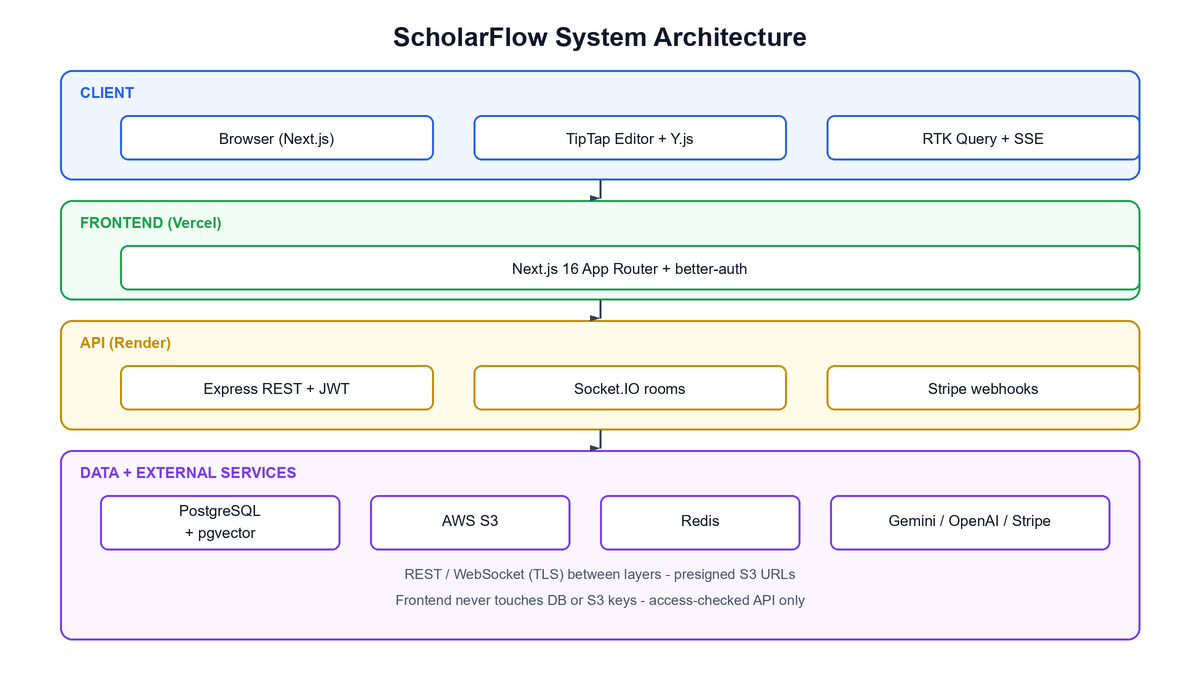
\includegraphics[width=0.95\textwidth]{figures/architecture.png}
\caption{ScholarFlow system architecture overview}
\label{fig:architecture}
\end{figure}

\subsection{Frontend Technologies}
Next.js 16 (App Router, Turbopack), React 19.2 + React Compiler (no manual
memoization), TypeScript strict, Tailwind CSS + shadcn/ui, RTK Query (all API
traffic; no raw fetch in components), React Hook Form + Zod, TipTap with
resizable-image, Y.js + socket.io client, Sonner toasts via provider helpers only.

\subsection{Backend Technologies}
Node.js $\geq$22, Express with TypeScript, strict Zod request validation,
thin controllers delegating to service-layer business logic, JWT with
bcrypt and refresh token rotation, rate limiting on mutations, Stripe SDK
for subscriptions and webhooks, Resend and SMTP email delivery, an hourly
node-cron sweeper, and Socket.IO rooms with JWT authentication.

\subsubsection{Backend File Structure}
The backend follows a modular feature architecture under \texttt{src/app/modules/}, isolating controllers, services, routes, and validation schemas:

\begin{verbatim}
backend/src/app/
|-- modules/
|   |-- Auth/         % JWT auth, bcrypt hashing, token rotation
|   |-- User/         % Profile management, credentials, preferences
|   |-- papers/       % Upload, S3 presigned URLs, metadata extraction
|   |-- annotations/  % PDF highlight marks, colors, and notes
|   |-- Workspace/    % Multi-tenant spaces, member roles, invitations
|   |-- Team/         % Lab collaborator management, role permissions
|   |-- AI/           % Multi-model LLM routing (Gemini/OpenAI/Claude)
|   |-- Search/       % pgvector HNSW cosine similarity search
|   |-- Billing/      % Stripe checkout, webhooks, portal, sweeper
|   |-- WebSocket/    % Socket.IO rooms, Y.js document synchronization
|   |-- Notification/ % Real-time SSE push streams, quiet hours
|   `-- Admin/        % System telemetry, user moderation, audit logs
|-- middleware/       % JWT verification, RBAC guards, rate limiters
`-- routes/           % Centralized REST route registration
\end{verbatim}

\subsection{Database Architecture}
Single shared PostgreSQL (Prisma Cloud) for dev and production; Prisma 7.8.0
with \texttt{@prisma/adapter-pg} pooling. Core ER model in
Fig.~\ref{fig:erd}: auth (User/Account/Session), collaboration
(Workspace/Member), library (Paper/File/Chunk, Collection), AI artifacts
(summaries, insight threads, embeddings). pgvector HNSW index
(\texttt{vector\_cosine\_ops}, m=16, ef\_construction=64); typed raw SQL only
for vector ops; one statement per file under \texttt{prisma/sql/}.

\begin{figure}[H]
\centering
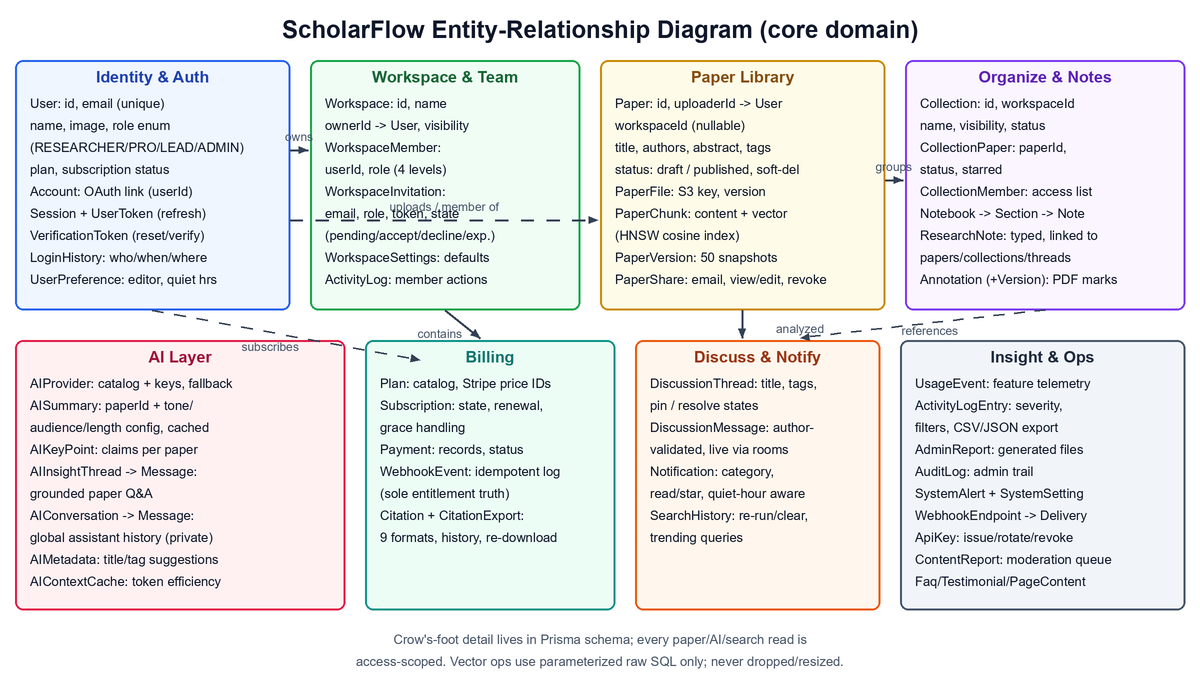
\includegraphics[width=0.95\textwidth]{figures/erd.png}
\caption{Entity--relationship diagram: full core domain (8 groups)}
\label{fig:erd}
\end{figure}

\subsection{AI and Machine Learning Integration}
Multi-provider service (Gemini primary, OpenAI/Claude/DeepSeek fallback),
embeddings pipeline with fixed-dimension validation and chunking, RAG-style
Q\&A over paper chunks, token-efficient context caching. Paper lifecycle in
Fig.~\ref{fig:lifecycle}.

\begin{figure}[H]
\centering
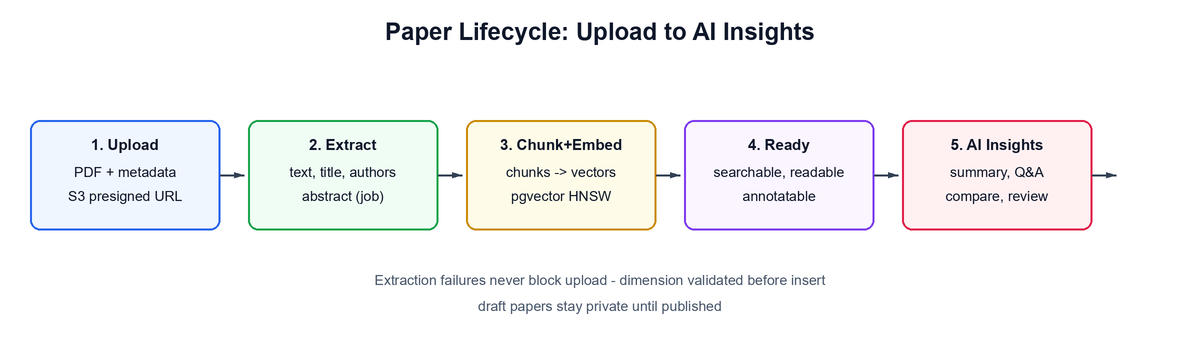
\includegraphics[width=0.9\textwidth]{figures/paper_lifecycle.png}
\caption{Paper lifecycle: upload, extraction, indexing, AI insights}
\label{fig:lifecycle}
\end{figure}

\subsection{Real-Time Communication Layer}
Dedicated Socket.IO server (Render) + in-app setup: JWT-verified handshake,
per-paper/discussion/workspace rooms, Y.js document sync, cursor presence,
typing indicators, late-joiner state sync, REST fallback when offline.

\subsection{Authentication and Security Architecture}
better-auth on the frontend paired with backend JWT authentication; OAuth
never overwrites user-customized profile names or avatars; RBAC via
\texttt{requireRole} after auth middleware; per-resource ownership checks in
services; presigned S3 URLs only; verified Stripe webhooks; admin-gated
metrics and team member search.

\subsection{External Integrations}
Google/GitHub OAuth, Gemini/OpenAI/Claude/DeepSeek AI, AWS S3, Stripe,
Resend/SMTP email, OpenAlex/arXiv scholarly feeds (TTL-cached, graceful
degradation).

\subsection{DevOps and Deployment Architecture}
Turborepo + Yarn Berry monorepo; Vercel (frontend), Render (API + socket
server); same Prisma Postgres for local and prod; GitHub Actions CI
(test + lint + type-check + build); health endpoints
(\texttt{/api/health}, \texttt{/detailed}, \texttt{/live}, \texttt{/ready}).

\subsection{Development and Testing Tools}
Jest + Supertest (21 suites / 59 tests, green), Playwright E2E, ESLint flat
configs, Prettier, Prisma Studio, Stripe CLI webhook forwarding, Repomix
snapshots.

\subsection{Key Technical Highlights}
\begin{itemize}[nosep]
\item Decoupled monorepo: frontend never imports backend/Prisma; REST only.
\item $<$50\,ms server-side query budget with slow-query terminal visibility.
\item Idempotent billing webhooks + sweeper (never webhook-only downgrades).
\item WCAG 2.1 AA, responsive 375\,px--desktop, dark mode.
\end{itemize}

\section{System Testing and Validation}
\begin{itemize}[nosep]
\item Auth: registration/login/logout, OAuth callbacks, JWT refresh, RBAC gates
  (403 on insufficient role), rate limiting on mutations.
\item Papers: upload validation (type/size), S3 presigned flow, metadata
  extraction fallback, draft/publish visibility, access-checked reads/writes.
\item Collaboration: invitations, role changes, email shares (view vs.\ edit),
  discussion threading, Y.js late-joiner sync.
\item Billing: CLI-forwarded webhooks (\texttt{checkout.session.completed},
  subscription events), idempotent replay, portal flows, sweeper downgrade.
\item AI: summary/Q\&A relevance review, 403 on unauthorized papers, escaped
  HTML rendering, provider fallback under outage.
\item API: Postman/Supertest contract checks; \texttt{yarn test} green
  (21 suites / 59 tests); lint + type-check clean; build green.
\end{itemize}
% TODO (fill-in): paste measured results (pass counts, latency samples, coverage).

\section{Challenges}
\begin{itemize}[nosep]
\item AI cost vs.\ quality: multi-provider routing, quotas, and caching to hold
  average AI cost under \$0.50/user/month without degrading summaries.
\item pgvector at latency distance: shared US-East cloud DB queried from
  Bangladesh ($\sim$100--250\,ms network-bound); adapter choice
  (\texttt{adapter-pg} pooling vs.\ HTTP) and select discipline keep deployed
  p95 under budget.
\item Migration drift: \texttt{db push} history bypasses vs.\ migration files;
  resolved via hand-written additive migrations + \texttt{migrate deploy}.
\item Auth-state races: redux-persist flush before hard navigation; better-auth
  client/server boundary (no \texttt{authClient} in client utilities).
\item Realtime durability: Y.js document seeding exactly once + debounced
  persistence so co-edits survive disconnects.
\end{itemize}
% TODO (fill-in): 1--2 lines each on what was tried and what finally worked.

\section{Future Enhancements}
\begin{itemize}[nosep]
\item Native mobile apps (web app is responsive; native is deferred).
\item Enterprise SSO/SAML, institution billing, IP allow-listing.
\item AI research-gap analysis and trend detection across collections.
\item Public API + plugin ecosystem (Overleaf/Word plugins, browser extension).
\item Offline-first editing with conflict resolution.
\item UI localization beyond English.
\end{itemize}

\section{Conclusion}
ScholarFlow demonstrates the application of software engineering principles ---
modular architecture, typed contracts, migration discipline, idempotent billing,
and measured quality gates --- to a real accessibility problem in academic
research. By unifying library management, AI analysis, academic writing, and
real-time collaboration at student-friendly pricing, the platform delivers a
scalable, secure foundation ready for pilot deployment and iterative growth.


% References
\begin{thebibliography}{9}
\bibitem{repo} ScholarFlow Repository.
  \url{https://github.com/Atik203/Scholar-Flow}
\bibitem{next} Next.js Documentation. \url{https://nextjs.org/docs}
\bibitem{express} Express.js Documentation. \url{https://expressjs.com/}
\bibitem{prisma} Prisma Documentation. \url{https://www.prisma.io/docs}
\bibitem{postgres} PostgreSQL Documentation. \url{https://www.postgresql.org/docs/}
\bibitem{pgvector} pgvector. \url{https://github.com/pgvector/pgvector}
\bibitem{s3} AWS S3 Documentation. \url{https://docs.aws.amazon.com/s3/}
\bibitem{stripe} Stripe Documentation. \url{https://stripe.com/docs}
\bibitem{gemini} Google Gemini Documentation. \url{https://ai.google.dev/docs}
\bibitem{openai} OpenAI Documentation. \url{https://platform.openai.com/docs}
\bibitem{srs} Phantom Devs. ScholarFlow Software Requirements Specification (SRS),
  United International University, Jan.\ 2026.
\end{thebibliography}


\end{document}
